\ifpdf
	\graphicspath{{2/pic/PNG/}{2/pic/PDF/}{2/pic/}}
\else
	\graphicspath{{2/pic/EPS/}{2/pic/}}
\fi

\chapter{Mathematical model of neutron transport}\label{chap:nte-review}

\nomenclature[s]{$f \approx g$}{$f$ is approximated by $g$}
\nomenclature[s]{$f \equiv g$}{$f$ is by definition equivalent to $g$}
\nomenclature[a]{$\R[n]$}{an n-dimensional Euclidean vector space}

The steady state neutron transport equation is a mathematical representation of balance between neutron gains and losses
within a given macroscopic domain $\VV\subset\R[3]$\index{D@$\VV$}. Let us consider the equation in its
integro-differential form with given neutron source function $q$\index{q@$q$}:
\begin{equation}\label{eq0}
  \begin{multlined}
    \Bigl[
      \bomega\cdot\grad + \sigma_t(\br,\bomega,E)
    \Bigr]
    \psi(\br,\bomega,E) =\\
    = \intE[']{\Emin}{\Emax}{\intA[']{\kappa(\br,\bomega\sla\bomega',E\sla E')\psi(\br,\bomega',E',t)}}  + 
    \src(\br,\bomega,E).
  \end{multlined}  
\end{equation}
Function $\sigma_t$\index{$\sigma_t$|see {cross-section: total}} groups all reactions that result in a loss of neutron,
while $\kappa$\index{$\kappa$} represents reactions that introduce neutrons into direction $\bomega$ and energy $E$ by,
e.g., scattering from direction $\bomega'$, slowing down (or accelerating) from higher (lower) energies $E'$ or releasing new neutrons from fissioned nuclei.
They are given by material composition of the domain and we will return to their more detailed description, as
well as to boundary conditions for \eqref{eq0}, in Section \ref{sec:NTE}.

Solution of eq. \eqref{eq0}, the \textit{angular neutron flux density} $\psi$\index{$\psi$|see {angular
flux}}\index{angular flux} -- is a function of the following independent variables, which define the neutron
phase space:
\begin{itemize}
 	\item $\br = (x,y,z)$	\index{r@$\br$}
 	\nomenclature[A]{\br}{position vector}
 	\nomenclature[U]{x,y,z}{components of vectors in Cartesian coordinate system} represents the spatial distribution of
 	 neutrons,
 	\item $\bomega$\nomenclature[g]{$\bomega$}{unit vector of neutrons flow direction}\index{$omega$@$\bomega$}
 	represents the angular distribution of neutrons on a unit sphere $\Sphere$\nomenclature[A]{\Sphere}{unit sphere ($\{x\in\R[3]: \norm{x} =
 	1\}$)}\index{S@$\Sphere$}, i.e. their streaming direction ($\bomega\in\R[3]$, $\norm{\bomega}=1$);
 	\item $E\in [E_{\text{min}},E_{\text{max}}]$\nomenclature[g]{$E$}{Energy of neutrons\nomunit{eV}}\index{E@$E$} is the
 	kinetic energy of neutrons.
\end{itemize}

\begin{remark}
	The phase space could be also defined in terms of the velocity vector $\bv$ and speed $v = \norm{\bv} = \sqrt{2E/m}$
	($m$ being neutron mass) instead of $\bomega$ and $E$. 
	This form appears to be preferred in analytical works, while our choice is more often used in practical numerical
	calculations.
	Corresponding changes in the formulation of the NTE are
	explicitly given e.g. in \cite[Chap. XXI, eqns. (1.1) and (1.2)]{DautrayLions}. For further use, we will just note
	that we can write $\bomega = \bv / v$ with $\bv\in\R[3]$\index{v@$\bv$, v}.
\end{remark} 
\begin{remark}
	In this macroscopic description, we should always consider beams of neutrons with the same average properties in
	differential elements around $\br$, $\bomega$, $E$. For simplicity, we will refer to them as to single neutrons with
	particular position, energy or direction (and occasionally call them $(\br,\bomega,E)$-neutrons) and we also omit the
	``density'' nomenclature of repeatedly used quantities -- e.g., we will henceforth call $\psi$ just \textit{angular
	neutron flux}.
\end{remark} 
\begin{remark}\label{rem:balance}
	We keep in mind that eq. \eqref{eq0} is a consequence of applying Gauss divergence
	theorem to the fundamental integral neutron balance over an arbitrary bounded subdomain of the phase space (which
	assumes differentiable angular neutron flux).
\end{remark}

\section{Neutron phase space} \label{sec:phase}
Let us assume that $\VV$ is a domain bounded by a piecewise smooth boundary $\pV$\index{Dp@$\pV$}, which is oriented
at almost every point $\br\in\pV$ (a.e. in $\pV$) by its unit outward normal field $\bn(\br)$\index{n@$\bn$}.
Then we may formally define the neutron phase space 
$$
  X \coloneqq \{(\br,\bomega,E):\ \br\in \VV\subset\R[3], \bomega\in \Sphere, E \in [\Emin,\Emax]\}
$$
\index{X@$X$} 
together with its outflow and inflow boundary subsets, respectively:
$$
  \pX[\pm] \coloneqq \bigl\{ (\br,\bomega,E) \in \pV \times \Sphere \times [E_m, E_M], \mbox{ s.t. }
  \bomega\cdot\bn(\br) \gtrless 0 \bigr\}.
$$
\index{Xp@$\pX[\pm]$, $\pX$} 
The whole boundary $\pX$ can be written as $$ \pX = \pX[+]\cup \pX[-] \cup \pX[0] $$ where $\pX[0]$ (boundary subset
tangential to the flow), so that $\overline X = X \cup \pX$.
\begin{figure}[!hbt]
    \centering 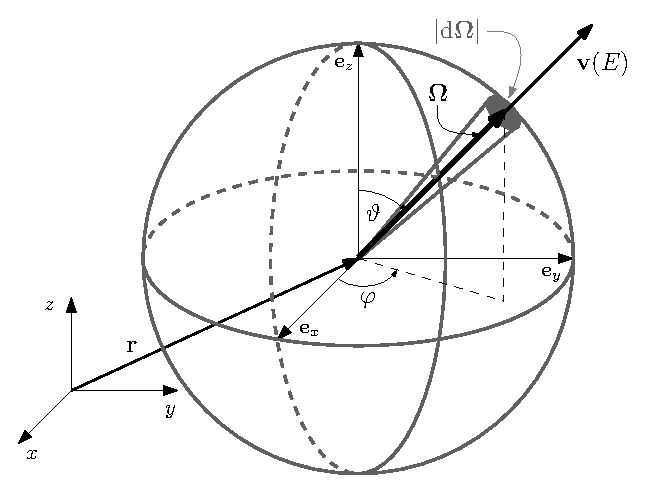
\includegraphics[scale=1]{phase_space.eps} \caption[Phase space of neutrons]{Phase space of neutrons}
    \label{fig:phase_space}
\end{figure}
The product Lebesgue measure
\begin{equation}\label{eq:measure}
  \d{x} = \d{\mu(X)} = \d{\mu(V\times\Sphere\times [\Emin,\Emax])} = \d{\br}\d{\bomega}\d{E}
\end{equation}
\index{dx@$\d{x}$}%
is used when integrating over $X$, 
while the boundary measure
\begin{equation}\label{eq:measure2}
\db = \abs{\bomega\cdot\bn}\d{S}\d{\bomega}\d{E},
\end{equation}
\index{dxi@$\db$}%
is used when integrating over $\pX[\pm]$, where $S = \mu(\pV)$.
Note that
because of the assumed regularity of the boundary, $\pX[0]$ is a closed subset of $\pX$ of
\linebreak\mbox{$\db$-measure} zero (\cite[Chap. XXI, Sec. 2.2]{DautrayLions}). This will allow us to decompose spaces 
of measurable functions defined on $\pX$ into a direct sum of subspaces of measurable functions defined on $\pX[+]$ and 
$\pX[-]$, respectively. When referring to physical units, we will consider the length scale of $\VV$ in centimeters.

\comment{
When discussing various semi-discretizations of the NTE, we will also refer to the following subspaces  (``sections''
through the phase space):
\begin{equation}\label{eq:pssec}
	X_E \coloneqq \{(\br,\bomega,E):\ \br\in \VV\subset\R[3], \bomega\in \Sphere, E \in [\Emin,\Emax]\}
\end{equation}
}

Since the direction vectors are confined to the sphere, we can express the three
Cartesian components of $\bomega$ by only two spherical coordinates $\polar\in[0,\pi]$ and
$\azimuthal\in[0,2\pi)$\nomenclature[g]{$\polar$}{polar angle}\nomenclature[g]{$\azimuthal$}{azimuthal
angle}:
\begin{equation*}
	\bomega = \left[\begin{array}{c}
		\Omega_x \\
		\Omega_y \\
		\Omega_z
	\end{array}\right] = \left[\begin{array}{c}
		\sint\cosp \\
		\sint\sinp \\
		\cost
	\end{array}\right]
\end{equation*}
(see \fref{fig:streaming}).\index{$omega$@$\bomega$}\index{$\vartheta$}\index{$\varphi$ (angle)}
\begin{figure}[!hbt]
    \centering
    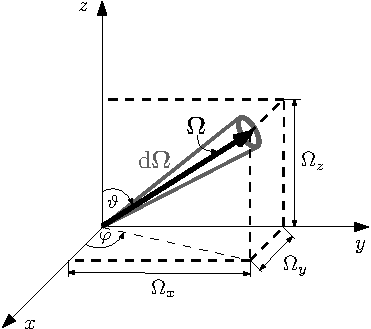
\includegraphics[scale=1.275]{cartesian_streaming}
    \caption[Cartesian coordinate system]{Cartesian coordinate system}
    \label{fig:streaming}
\end{figure}
To transform integrals with respect to $\d{\bomega}$ into double integrals with respect to $\polar$ and $\azimuthal$,
note that the solid angle $\d{\bomega}$ subtended at the center of $\Sphere$ by the spherical differential element
$\abs{\d{\bomega}}$ can be written as:
$$
	\d{\bomega} = \frac{\abs{\d{\bomega}}}{r^2} = \frac{r^2 \sint \d{\polar}\d{\azimuthal}}{r^2} =  \sint
	\d{\polar}\d{\azimuthal} $$
(see \fref{fig:element}).\index{$\d{o}$@$\d{\bomega}$}
\begin{figure}[!hbt]
    \centering
    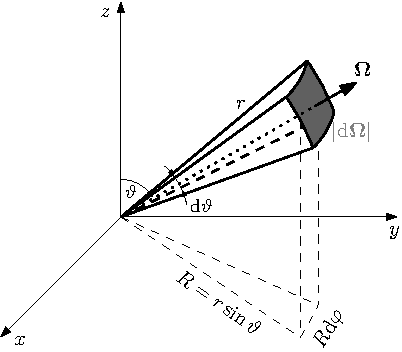
\includegraphics[scale=1.275]{element}
    \caption[Solid angle]{Schematic view of the solid angle of directions}
    \label{fig:element}
\end{figure}
We will also need to integrate functions that depend on the cosine of the angle between two 
directions $\bomega$ and $\bomega'$. We shall denote this angle and its cosine by $\polar_0$ and $\mu_0$, respectively
(see \fref{fig:scatter} in appendix for geometrical interpretation).
Then
$$
	\mu_0 \equiv \cos \polar_0 = \bomega\cdot\bomega'
$$
\index{$\mu_0$}
and
\begin{equation}\label{eq:invint}
\begin{aligned}
	\intA[']{f(\bomega\cdot\bomega')} &= \int_{0}^{2\pi} \int_{0}^{\pi}
		f(\cos \polar_0) \sin \polar_0\d{\polar_0} = 2\pi \muint[_0]{f(\mu_0)}\\
		&= \intA{f(\bomega'\cdot\bomega)}
\end{aligned}
\end{equation}
Notice that the result depends on neither $\bomega$ nor $\bomega'$.

\section{Steady state neutron transport in isotropic bounded domain}\label{sec:NTE}
In most practical cases, we can assume that the medium in which we study neutron transport is isotropic.
The first consequence of this assumption is that 
$$
	\sigma_t(\br,\bomega,E)\psi(\br,\bomega,E) \equiv \sigma_t(\br,E)\psi(\br,\bomega,E)
$$ 
for all $\br$, $\bomega$, $E$. The
second is that reactions that change the direction of neutrons from $\bomega'$ to $\bomega$ are
invariant under rotation of the coordinate system and are thus completely determined by the cosine of the two vectors:
\begin{equation}\label{eq:iso}
	\kappa(\cdot,\bomega\sla\bomega',\cdot) \equiv \kappa(\cdot,\bomega\cdot\bomega',\cdot).
\end{equation}
The steady state NTE \eqref{eq0} in this regime reads
\begin{equation}\label{eq1}
\begin{multlined}
  \bomega\cdot\nabla\psi(\br,\bomega,E) + \sigma_t(\br,E)\psi(\br,\bomega,E) =\\[.25em]
   = \intE[']{\Emin}{\Emax}{
      \intA[']{\kappa(\br,\bomega\cdot\bomega',E\sla E')\psi(\br,\bomega',E')}
    } + q(\br,\bomega,E)
 \end{multlined}
\end{equation}
in $X$, complemented by specified angular flux distribution at $\pX[-]$. The two prototypical inflow boundary
conditions are:\index{boundary conditions}
\begin{itemize}
	\item incoming angular neutron flux
	\begin{equation}\label{eq:nte2}
	  \psi\vert_{\pX[-]} = \psi_{\text{in}}
	\end{equation}\index{$\psi\vert_{\pX[\pm]}$}%
	($\psi_{\text{in}}\equiv 0$ corresponds to vacuum in $\R[3]\setminus \overline V$, which is a common
	 assumption in nuclear reactor modeling),%
	 \index{boundary conditions!vacuum}%
	
	\item albedo boundary reflection
	\begin{equation}\label{eq:nte3}
  	\psi(\br,\bomega,E) = \albedo(\br)\psi(\br, \bomega_R, E),\quad (\br,\bomega,E)\in \pX[-],\ \ \bomega_R = \bomega - 2
  	\bn (\bomega \cdot \bn)
  \end{equation}\index{$omegaR$@$\bomega_R$}\index{$\beta$|see {boundary conditions:
  albedo}}\index{boundary conditions!albedo}\index{boundary conditions!reflective}%
  where $\bomega$ is the reflection of
  $\bomega_R$ about the boundary plane. For $\albedo \equiv 1$, this corresponds to complete specular reflection and is used to model planes of symmetry, while for $\albedo \equiv 0$, we recover the vacuum condition from above. Intermediate values mean that a fraction of neutrons leaving the domain in direction $\bomega_R$ are returned back in direction $\bomega$, which is commonly used to model reactor
  reflectors. We thus assume $0 \leq \albedo \leq 1$. 
\end{itemize}
\begin{remark}
	The albedo coefficient $\albedo$ may in general vary with the reflector properties and should also capture 
	redistribution of the reflected neutrons within the phase space due to their diffusion through the reflector. A general
	treatment of albedo condition is given in \cite{Sanchez4} (see also \cite{Sanchez3}), where an integral albedo operator
	$\albedoop$ is introduced, such that
\begin{equation}\label{eq:albedo-general}
	\angflux(x)\big\vert_{\pX[-]} = (\albedoop\angflux)(x) = \bndint[']{\pX[+]}\albedo(x\sla x')\angflux(x'),
\end{equation}
	where $x = (\br,\bomega,E)$ and $x' = (\br',\bomega',E')$.
	\index{operator!B@$\albedoop$}%
\end{remark}
For formal description of other types of boundary conditions, we refer to \cite{Sanchez4} or \cite[Sec. 1.3]{Agoshkov}.

A physically plausible solution of the NTE should be moreover non-negative throughout $\VV$ and continuous along any
direction $\bomega$, i.e. $\psi(\br + s\bomega,\bomega,E)$ is a continuous function of $s$ for any $\br$, $\bomega$, $E$. Note
that $\psi(\br + s\bomega',\bomega,E)$ \textsl{may} be discontinuous as a function of position when $\bomega' \neq
\bomega$.

\subsection{Advection term}\label{sec:advection}
In Cartesian coordinate system (that we will exclusively consider in this thesis),
$$
	\bomega\cdot\nabla\angflux = \bomega_x\pd{\angflux}{x} + \bomega_y\pd{\angflux}{y} + \bomega_z\pd{\angflux}{z} = 
	\der{x}{s}\pd{\angflux}{x} + \der{y}{s}\pd{\angflux}{y} + \der{z}{s}\pd{\angflux}{z} = \der{\angflux}{s},
$$
where $s\in I\subset \R$ parametrizes the path traveled by the neutron along the direction $\bomega$ (the
\textit{characteristic}, see \fref{fig:cartesian2}).
\begin{figure}[btp]
\begin{center}
  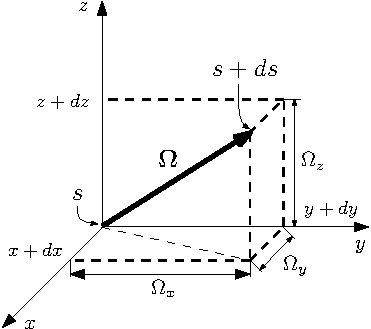
\includegraphics[scale=1.2]{cartesian_streaming2}
  \caption{Characteristic direction in the Cartesian coordinate system}
  \label{fig:cartesian2}
\end{center}
\end{figure}
\index{characteristic}
Assuming now for simplicity that the integral term on the right of \eqref{eq1} is absorbed in the source term
$q$, we may invert the differential operator on the left of \eqref{eq1} by integration along these characteristics and obtain an
integral formulation of the neutron transport equation:
\begin{equation}\label{eq:nte-integral}
	\angflux(\br,\bomega) = \angflux(\br_0,\bomega)e^{-\tau(\br,\br_0)} + \int_0^{s_0}
	q(\br',\bomega)e^{-\tau(\br,\br')}\,\d{s'}
\end{equation}
where
\begin{align}
	\br' &= \br - s' \bomega, \quad \br_0 = \br - s_0 \bomega\nonumber\\[.2em]
	\tau(\br,\br') &= \tau(\br,\br-s'\bomega) = \int_0^{s'} \sigma_t(\br - s''\bomega)\,\d{s''} \label{eq:tau}
\end{align}
\index{$\tau(\br,\br')$}%
In reference to \fref{fig:trepka}
\begin{figure}[tbp]
\begin{center}
  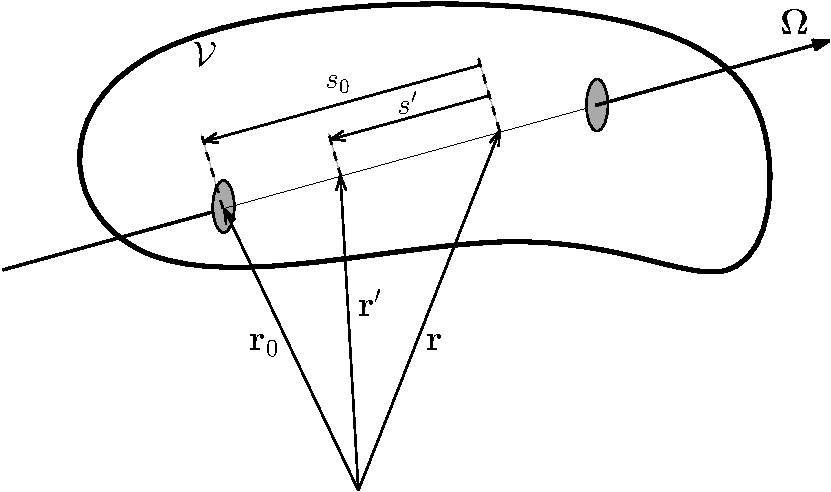
\includegraphics[scale=.75]{trepka}
  \caption{Illustration for the solution on a characteristic}
  \label{fig:trepka}
\end{center}
\end{figure}
\index{l@$\ell$}
we can interpret the first term on the right of \eqref{eq:nte-integral} as the number of
neutrons moving in the direction $\bomega$ that entered the given volume at $\br_0$ and reached point $\br$ without
collision, whereas the second term as the number of neutrons introduced into the characteristic direction by sources 
between $\br_0$ and $\br$ and reaching $\br$ without collision. The \textit{optical path length} $\tau$ represents the 
probability of collision between $r'$ and $r$. This integral form is of both theoretical and practical value, as we will
see later in sections \ref{sec:fixed-source} and \ref{sec:lattice}.

\subsection{Collision terms}
\index{cross-section}
The kernel of the integral operator on the right-hand side of \eqref{eq1} characterizes the mean number of
($\bomega$,~$E$)-neutrons coming out of a collision of ($\bomega'$,~$E'$)-neutrons with nuclei at $\br$ (or more
precisely in a differential element around $\br$). Such collisions can either just change the direction and energy of
the inducing neutrons (elastic scattering)\index{scattering!elastic} or cause absorption of the neutrons followed by
release of new ones in the considered direction and energy range (fission), or both (inelastic
scattering)\index{scattering!inelastic}.
This categorization motivates the splitting
\begin{equation}\label{eq:splitting}
  \kappa(\br,\bomega\cdot\bomega',E\sla E') = \eta\sigma_s(\br,\bomega\cdot\bomega',E\sla E') +
  \nu\sigma_f(\br,\bomega\cdot\bomega',E\sla E').
\end{equation}
where the two components are the so-called \textit{double-differential macroscopic
cross-section}\index{scattering!double-differential} for scattering and fission, respectively. 
The \textit{scattering} and \textit{fission yield} $\eta$ and $\nu$\index{$\eta$}\index{$\nu$|see
{fission yield}}\index{$\sigma_s$|see {cross-section: scattering}}\index{$\sigma_f$|see {cross-section:
fission}}\index{cross-section!fission}\index{cross-section!scattering}, respectively, have the meaning of expected
number of neutrons coming out of the scattering event ($=1$ in case of elastic scattering, might be $> 1$ when inelastic
scattering takes place) and the fission event, respectively, per one inducing neutron.
% As they will always appear in the product with the appropriate cross-section, their dependence on $\br, E', \bomega'$ is omitted. 

Ordinary macroscopic cross-sections $\sigma_s(\br,E)$,
$\sigma_f(\br,E)$ are then introduced to characterize the total probability that $(\bomega,E)$ neutrons undergo 
collisions of the above type irrespective of the outgoing (primed) direction and energy\footnote{Recall that the
direction $\bomega$ of the incoming neutrons is irrelevant for the result as a consequence of the assumption of isotropic medium (and eq. \eqref{eq:invint}).}, i.e.
\begin{equation}\label{eq:ddifxs}
\begin{aligned}
\eta\sigma_s(\br, E) &=
\intE[']{\Emin}{\Emax}{\intA[']{\eta\sigma_s(\br,\bomega'\cdot\bomega, E'\sla E)}},\\
\nu\sigma_f(\br, E) &= \intE[']{\Emin}{\Emax}{\intA[']{\nu\sigma_f(\br,\bomega'\cdot\bomega, 
	E'\sla E)}}.
\end{aligned}
\end{equation}

The \textit{total macroscopic cross-section}, $\sigma_t$\index{cross-section!total}, characterizing the probability
that neutron with energy $E$ undergoes a collision of any type with nuclei at $\br$, can now be decomposed as 
\begin{equation}\label{eq:st}
  \sigma_t(\br,E) = \sigma_c(\br,E) + \sigma_f(\br,E) + \sigma_s(\br,E) \equiv \sigma_a(\br,E) + \sigma_s(\br,E)
\end{equation}
where
\begin{itemize}
	\item $\sigma_c(\br, E)$ is the non-productive capture cross section (resulting in no new neutrons being introduced
	into the system) and
  	\item $\sigma_a(\br, E) = \sigma_c(\br,E) + \sigma_f(\br,E)$ is the absorption cross section.
\end{itemize}
\index{$\sigma_c$|see {cross-section: capture}}\index{cross-section!capture}
\index{$\sigma_a$|see {cross-section: absorption}}\index{cross-section!absorption}

For later use, note that fission is an isotropic process (which removes the angular dependence of the
double-differential fission cross-section altogether) and the new energy distribution does not depend on energy of 
the inducing neutron 
\begin{figure}[hbt]
\begin{center}
  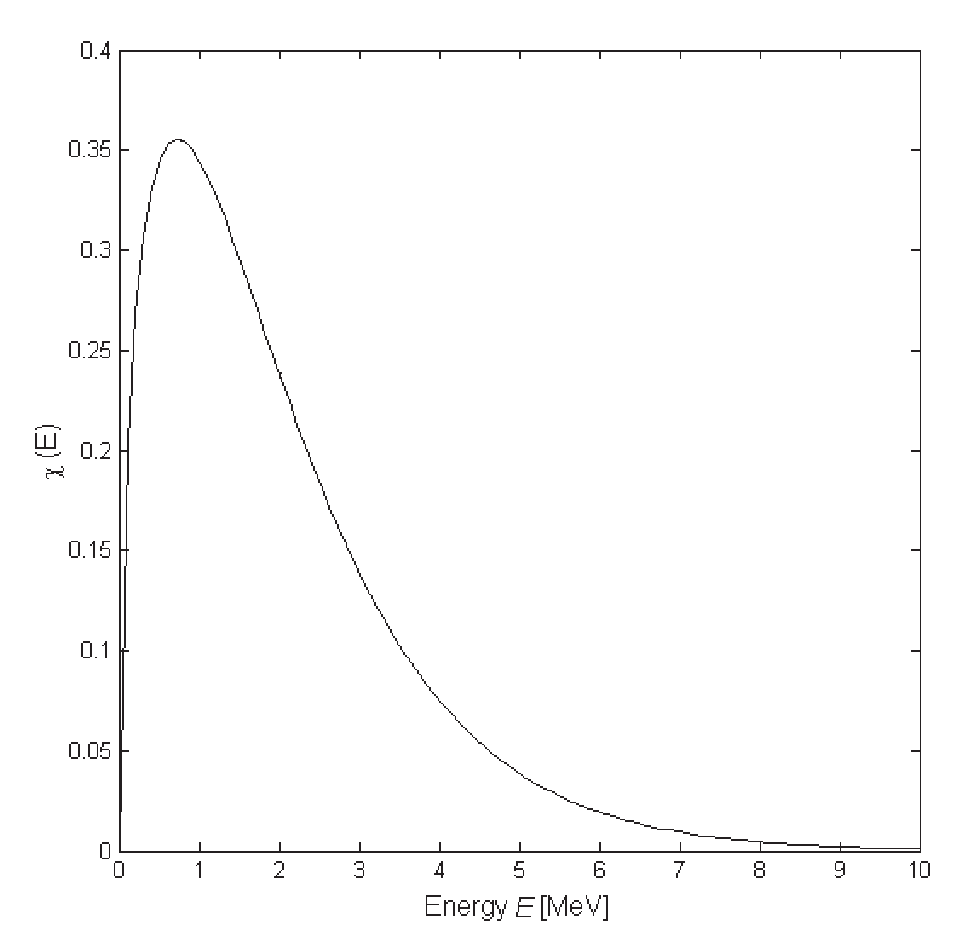
\includegraphics[scale=.6]{spectrum}
  \caption{Energy spectrum of (prompt) neutrons released from fission of U235}
  \label{fig:spectrum}
\end{center}
\end{figure}
(as it corresponds to neutrons originally bound inside the nucleus; \fref{fig:spectrum}
shows a typical shape of that function); using the second eq.
\eqref{eq:ddifxs}, we can then write:
\begin{equation}\label{eq:sf}
\nu\sigma_f(\br,\bomega\cdot\bomega',E\sla E') \equiv \frac{\chi(E)\nu\sigma_f(\br,E')}{4\pi},\quad 
\intE{\Emin}{\Emax}{\chi(E)} = 1.
\end{equation}
\index{$\chi$|see {fission spectrum}}\index{fission spectrum}
 
A physically realistic assumption is that all the macroscopic cross-sections are bounded measurable functions\footnote{
with respect to product measure of type \eqref{eq:measure} appropriate for their particular set of arguments, or with  
respect to $\d{\mu(V\times\Sphere^2\times [\Emin,\Emax]^2)}$ in case of double-differential cross-section}, piecewise 
continuous in $\VV$. The unit of macroscopic cross-sections is \SI{}{cm^{-1}}.

\subsection{Quantities of interest}\label{sec:qoi}
From the solution of eq. \eqref{eq1}, one can derive the following important integral quantities
\begin{itemize}
  \item \textit{scalar neutron flux (density)} \SI{}{[cm^{-2}.s^{-1}]}
  \begin{equation}\label{eq:scalar_flux}
    \phi(\br, E) = \intA{\psi(\br,\bomega,E)},
  \end{equation}
  \index{$\phi$|see {scalar flux}}\index{scalar flux}
  \item \textit{net neutron current (density)} \SI{}{[cm^{-2}.s^{-1}]}
	\begin{equation}\label{eq:bJ}
		\bJ(\br, E)	= \intA{\bomega\psi(\br,\bomega,E)},
	\end{equation}
	\index{J@$\bJ$|see {net current}}\index{net current}
\end{itemize}
so that integrating $\bJ(\br,E)\cdot\bn(\br)$ over a given surface 
gives the total number of neutrons with energy $E$ crossing (per unit time) that surface in the direction of 
$\bn$ (and allows assessing neutron conservation within given volume, recall Remark~\ref{rem:balance}).

The integral
\begin{equation}\label{eq:rr}
  \intE{E_1}{E_2}{\sigma_x(\br, E) \phi(\br, E)}
\end{equation}
represents the \textit{reaction rate density} (per unit time)\index{reaction rate} of given type ($x = t,a,f,s,c$, see
\eqref{eq:st}), induced by neutrons of energies in range $[E_1, E_2]$. 
As well as the scalar flux itself, reaction rates may be experimentally measured
by various detector mechanisms, which is the reason why these quantities are more important in practical calculations
than the actual solution of the NTE (angular neutron flux $\psi$). Of particular importance for reactor calculations is
the
\textit{power density} 
\begin{equation}\label{eq:power}
	P(\br) = \intE{\Emin}{\Emax}{e\sigma_f(\br, E) \phi(\br, E)} \quad \SI{}{[W.cm^{-3}]}
\end{equation}
where $e$ is the energy conversion factor converting fission rate to watts.
\index{P@$P$|see {power density}}

\subsection{Solvability of neutron transport problems}\label{sec:ntp}
In this section, we will formulate two basic problems of neutron transport in an operator form.
We will be interested in \textit{generalized solutions} of these problems (which we call just solutions), which satisfy
the equation and boundary conditions almost everywhere (a.e.) in $X$ (or $\pX$), and understand by $\bomega\cdot\nabla$
the generalized directional derivative in the usual Sobolev sense. This is motivated by the low regularity that can be
expected from the exact solution of the NTE -- for example, even for piecewise smooth material data  (cross-sections
$\sigma_x$) and sources $q$, the solution of the NTE is known to possibly exhibit singularities in first partial 
derivatives (or be discontinuous as a function of $\bomega$) at surfaces of material discontinuities coinciding with 
characteristic curves of the left-hand side of \eqref{eq1} (that is, straight lines; see \cite[Chap.
1]{Agoshkov}, \cite[Sec. III]{Vladimirov}).
% We will call the solution of such a generalized problem a \textit{weak solution}.



\subsection{Neutron transport problem with fixed sources}\label{sec:fixed-source}
Let us introduce the standard spaces of Lebesgue-integrable functions (w.r.t. the product measure \eqref{eq:measure},
resp. \eqref{eq:measure2}) 
\begin{equation}\label{eq:Lp}
\nomenclature[a]{$\Lp(X)$}{space of functions integrable in the Lebesgue sense with their $p$-th power over
$X$\nomrefeq}
\nomenclature[a]{$\Lp_\sigma(X)$}{space weighted with the total cross-section $\sigma_t$\nomrefeq}
\begin{aligned}
	\Lp(X) &= \left\{\psi\mid \norm[\Lp(X)]{\psi} \coloneqq \left(\int_X\abs{\psi(x)}^p\,\d{x}\right)^{1/p} <
	\infty\right\},\quad 1\leq p < \infty,\\
	\Lp(\pX[\pm]) &= \left\{\psi\mid \Vert\psi\Vert_{\Lp(\pX[\pm])} \coloneqq
	\left(\int_{\pX[\pm]}\abs{\psi(x)}^p\,\db\right)^{1/p} < \infty\right\},\quad 1\leq p < \infty,\\
	\Lp[\infty](X) &= \{\psi\mid \norm[L^{\infty}(X)]{\psi} \coloneqq \esssup_{X} \abs{\psi(x)} < \infty\}\\
	\Lp[\infty](\pX[\pm]) &= \{\psi\mid \Vert\psi\Vert_{L^{\infty}(\pX[\pm])} \coloneqq \esssup_{\pX[\pm]}
	\abs{(\bomega\cdot\bn)\psi(x)}< \infty\}
\end{aligned}
\end{equation}
Note that for the total volumetric scalar flux to be finite  (as is physically expected), the solution should belong to
$\Lp[1](X)$.
\index{space!$\Lp(X)$}\index{space!$\Lp[\infty](X)$}\index{space!$\Lp(\pX[\pm])$}\index{space!$\Lp[\infty](\pX[\pm])$}

We formulate the fixed source problem using the following operators:
\begin{equation*}
  \begin{gathered}
    A\psi(\br,\bomega,E) = \bomega\cdot\nabla\psi(\br,\bomega,E),\\%[.85em]
    \Sigma_t\psi(\br,\bomega,E) = \sigma_t(\br,E)\psi(\br,\bomega,E),\\%[.75em]
    K\psi(\br,\bomega,E) = \intE[']{\Emin}{\Emax}{
            \intA[']{\kappa(\br,\bomega\cdot\bomega',E\sla E')\psi(\br,\bomega',E')}
          }.
  \end{gathered}
\end{equation*}
We shall call $A$, $\Sigma_t$, $K$ and $T = A + \Sigma_t - K$ the \textit{advection}, \textit{reaction}, 
\textit{collision} and \textit{transport} operator, respectively. All these operators are continuous; the reaction
operator $\Sigma_t : \Lp(X) \to \Lp(X)$ is a simple multiplication operator in $\Lp(X)$, self-adjoint and bounded,
while the operator $K: \Lp(X) \to \Lp(X)$ is bounded under additional (physically justifiable) conditions
(conditions (c) and/or (d) of the following theorem, depending on $p$), but is self-adjoint if and only 
if the kernel $\kappa$ of $K$ is symmetric in $E$ and $E'$. With the exception of the mono-energetic case, this is
generally not true (a fact to which we return again in \sref{sec:MG}). To further simplify notation, let us also define 
$$
	\op{L} \coloneqq A + \Sigma_t.
$$
\index{operator!L@$\op{L}$}\index{operator!A@$A$}\index{operator!S@$\Sigma_t$}\index{operator!K@$K$}\index{operator!T@$T$}%
For piecewise smooth
$\pV$ and $1\leq p < \infty$, the traces $\Gamma_{\pm}\psi \equiv
\psi\vert_{\pX[\pm]}\in\Lp(\pX[\pm])$\index{$\psi\vert_{\pX[\pm]}$} are well defined for functions  $\psi\in \widehat
H^p(X)$, where $$
\widehat H^p(X) = \{\psi\mid \psi\in\Lp(X), \bomega\cdot\nabla\psi\in\Lp(X)\}, \quad 1 \leq p \leq \infty
$$
and a continuous lifting operator 
$$
	\mathcal{G}: \psi_{\pm}\in\Lp(\pX[\pm]) \mapsto \widehat\psi \in \widehat H^p(X)
$$
such that $\widehat\psi\vert_{\pX[\pm]} = \psi_{\pm}$ exists (\cite[Thm. 1, Appendix of \S 2, Chap.
XXI]{DautrayLions}, \cite{Boulanouar1} for the case $p = \infty$).
The Sobolev space of functions with bounded boundary traces is then defined as
\begin{equation}\label{eq:Hp}
  \nomenclature[a]{$\Hp{p}(X)$}{Sobolev space of functions whose (generalized) partial derivatives up to order $k$ are
 in $\Lp{p}$.\nomrefeq} 
 \Hp(X) \coloneqq \left\{\psi\in\Lp(X), \bomega\cdot\nabla\psi\in\Lp(X), \Vert\Gamma\psi\Vert_{\Lp(\pX)} < \infty\right\}. 
\end{equation}
\index{space!$\Hp(X)$}%
and $A : \Hp(X) \to \Lp(X)$, thus the complete transport operator \linebreak\mbox{$T: \Hp(X) \to \Lp(X)$}.
We note that $\Hp[2](X)$ is a Hilbert space when equipped with the inner product
\begin{equation*}\label{eq:ip}
	\ip{\Hp[2](X)}{\psi,\varphi} \coloneqq \ip{\Lp[2](X)}{\bomega\cdot\nabla \psi, \bomega\cdot\nabla \varphi} +
	\ip{\Lp[2](X)}{\psi,\varphi} +
	\ip{\Lp[2](\pX)}{\psi,\varphi} 	
\end{equation*}
\index{$z$@$\ip{\Hp[2](X)}{\cdot,\cdot}$}where
\begin{equation}\label{eq:ipL2}
	\ip{\Lp[2](X)}{\psi,\varphi} = \int_X \psi \varphi \,\d{x},\quad
	\ip{\Lp[2](\pX)}{\psi,\varphi} = \int_{\pX} \psi \varphi \,\d{\xi}.
\end{equation}
\index{$z$@$\ip{\Lp[2](X)}{\cdot,\cdot}$}\index{$z$@$\ip{\Lp[2](\pX)}{\cdot,\cdot}$}

\index{boundary conditions}
The lifting operator allows us to pick a function $\widehat \psi = \mathcal{G}\psi_{\text{in}} \in \Hp(X)$ and convert a
problem $T\psi = q$ with non-homogeneous boundary conditions \eqref{eq:nte2} to a problem 
$$
	T(\psi - \widehat\psi) = q - T\widehat\psi \equiv \widehat q
$$ 
where trace of the new unknown function $u = \psi - \widehat\psi$ on $\pX[-]$ vanishes. Final solution is then recovered
as $\psi = u + \widehat{q}$. Therefore, we can focus on the case with homogeneous conditions and put $\Dom{T} =
\Hpnot(X)$ where
$$
	\Hpnot(X) \coloneqq \{\psi\in \Hp(X),\ \psi\vert_{\pX[-]} = 0\}.
$$
\index{space!$\Hpnot(X)$}%
Similar treatment of reflective or more general boundary conditions requires special trace theorems, see
\cite[Chap. XXI, Appendix of \S2]{DautrayLions} or \cite[Chap. 2]{Agoshkov}.

The fixed source, steady state neutron transport problem with vacuum boundary conditions that we are going to study in
this section is posed as follows

\begin{problem}\label{prb:1}
For given $q\in \Lp(X)$ find $\psi \in \Hpnot(X) \subset \Lp(X)$ such that
$
     T\psi = q.
$
\end{problem}
\index{problem!fixed-source}

We will first consider the physically most natural $\Lp[1](X)$ case.

\subsubsection{$\Lp[1](X)$ setting}
\begin{theorem}\label{thm1}
Assume that
\begin{enumerate}[label=(\alph*)]
	\item $\sigma_t \in \Lp[\infty](X)$, $\sigma_t \geq \mst > 0$ a.e. in $\VV\times[\Emin,\Emax]$,
	\item $\kappa \geq 0$ a.e. in $\VV\times\Sphere^2\times[\Emin,\Emax]^2$,
	\item $\displaystyle c \leq \bar c < 1$ a.e. in $\VV\times[\Emin,\Emax]$ where
	  \begin{equation}\label{eq:c}
	    c(\br,E) \coloneqq \frac{1}{\sigma_t(\br,E)}\int_{\Emin}^{\Emax}\int_{\Sphere} \kappa(\br,\bomega'\cdot\bomega,
	    E'\sla E)\,\d{E'}\d{\bomega'}.
	  \end{equation}
\end{enumerate}
Then Problem \ref{prb:1} with $p = 1$ has a unique solution $\psi\in\Hpnot[1](X)$.
\end{theorem}
\begin{proof}
\cite[Chap. XXI, \S 2, Proposition 5]{DautrayLions}
\end{proof}

The value $c$ in Thm. \ref{thm1} has the physical meaning of the mean (net) number of neutrons emitted (in all possible
directions and energies) per a neutron with energy $E$ (coming from any direction) colliding with a nucleus at point
\mbox{$\br\in V$}. 
Condition (c) thus expresses the requirement that the system be \textit{subcritical} in order for a
steady solution in presence of external sources to be achieved (the notion of criticality will be formally introduced in the following
subsection).
Notice that (using \eqref{eq:ddifxs})
\begin{equation}\label{eq:scattering_ratio}
	c(\br,E) = \frac{\eta\sigma_s(\br,E) + \nu\sigma_f(\br,E)}{\sigma_t(\br,E)}
\end{equation}
and is usually called \textit{collision ratio} \index{c|see{collision ratio}}\index{collision ratio} (or
\textit{scattering ratio} in non-fissioning domains)\index{scattering ratio}.
\index{subcritical}
\index{characteristic}

 In \cite{Sanchez3}, Sanchez uses the inversion of the transport operator along characteristics (see \ref{sec:advection}
 above) to prove existence and uniqueness of solution to the fixed source neutron transport problem in
 the cross-section weighted space $\Hp[1]_{\sigma}(X)$ for right hand sides in $\Lp[1]_{\sigma}(X)$ (and albedo
 boundary conditions of general type
 \eqref{eq:albedo-general}).\index{space!$\Lp[1]_{\sigma}$}\index{space!$\Hp[1]_{\sigma}$}%
 This appears to be an alternative physically natural functional setting due to the definition of reaction rate, eq. 
 \eqref{eq:rr}; moreover, assumption (a) may be relaxed by allowing $\sigma_t = 0$ in arbitrarily large regions 
  (the \textit{void regions})\index{void regions}. Note that if we assume (a) of Thm. \ref{thm1}, the norms of $\Lp[1]$
  and $\Lp[1]_{\sigma}$ are equivalent and the measure $\d{\tau} = \sigma_t(x) \d{x}$ associated with the space
  $\Lp[1]_{\sigma}$ represents a differential optical path length (see eq. \eqref{eq:tau}).

\subsubsection{$\Lp[\infty](X)$ setting}
In \cite[Chap. XXI, \S 2, Proposition 6]{DautrayLions}, Dautray and Lions also 
show the existence of unique solution in $\Lp[\infty](X)$ for $q\in \Lp[\infty](X)$; the proof in this case is again
based on the inversion of the transport operator along characteristics and requires instead of
 (c) the condition
\begin{enumerate}
  \item[(d)] $d \leq \overline d < 1$ a.e. in $\VV\times[\Emin,\Emax]$
\end{enumerate}
where
\begin{equation}\label{eq:d} 
d(\br,E) \coloneqq 
  \frac{1}{\sigma_t(\br,E)}\int_{\Emin}^{\Emax}\int_{\Sphere} \kappa(\br,\bomega\cdot\bomega',
	    E\sla E')\,\d{E'}\d{\bomega'}
\end{equation}\index{d}%
can be interpreted as the average number of neutrons emitted with energy $E$ from
collisions induced by all possible neutrons impinging on the nucleus at $\br$ (again, this is a reasonable condition
in the subcritical state). Notice that because angular dependence of $\kappa$ is only through the cosine of the
collision angle (i.e., $\bomega\cdot\bomega'$), the outgoing direction is immaterial and assumptions (c) and (d) really
represent different assumptions about just the energy transfer in collisions. 

\subsubsection{$\Lp[2](X)$ setting and second-order forms of NTE}\label{sec:L2}
In general $\Lp(X)$ spaces with $1 < p < \infty$, Dautray and Lions outline the proof based on the same ideas as those
used in the $\Lp[1](X)$ case (theory of monotone operators), utilizing assumptions (a-d) of Thm. \ref{thm1}.  The case
$p = 2$ is particularly important
%\footnote{even though it does not lead to a direct physical interpretation as  the
%$\Lp[1](X)$ setting} 
as the Hilbert space structure of $\Lp[2](X)$ allows to use richer set of mathematical tools to
formulate practical solution methods. In particular, it allows to formulate variational principles for the NTE, which
are of both theoretical and practical importance. 

Let us set $V = \Hpnot[2](X)$ and let $V'$
denote the dual space, i.e.
the space of bounded linear functionals on $V$\index{space!dual}.  For $T : V \to V'$, we may view the problem of
finding $\psi \in V$ such that $T\psi = q$
as a problem posed in $V'$ and write it in the variational (or \textit{weak}) form: Find $\psi \in V$ such that 
\begin{equation}\label{eq:weakform0}
	\langle T\psi, \varphi \rangle = \langle q, \varphi \rangle  \quad \forall \varphi\in V,
\end{equation}
where $\langle \cdot,\cdot\rangle$ denotes the duality pairing between $V'$ and $V$. As usual, we will refer to the
arbitrarily varying functions $\varphi\in V$ in \eqref{eq:weakform0} as to \textit{test functions}.
\index{$\varphi$ (test function)}

This formulation
allows considering more general right hand sides \linebreak\mbox{$q \in V' \supset \Lp[2](X)$}, but we will restrict our
attention to the case represented by Problem \ref{prb:1} with $p = 2$, i.e. $T : V \to \Lp[2](X)$ with $q \in
\Lp[2](X)$.  Since for $\Lp[2](X)$ the duality pairing coincides with the ordinary $\Lp[2](X)$ inner product
\eqref{eq:ipL2} and the Riesz representation theorem lets us identify $\Lp[2](X)$ with its dual, we also identify the
linear functionals $Tu,q \in [\Lp[2](X)]'$ with their Riesz representants $Tu,q \in \Lp[2](X)$. If we now define
the bilinear and linear form $$ a(u,v) = \ip{\Lp[2](X)}{Tu,v}, \quad f(v) = \ip{\Lp[2](X)}{q,v}, $$
we can write the weak formulation \eqref{eq:weakform0} as
\begin{problem}\label{prb:2}
For given $q\in \Lp[2](X)$ find $\psi \in V$ such that
$$
	a(\psi, \varphi) = f(\varphi) \quad \forall \varphi\in\Lp[2](X).
$$
\end{problem}
\index{problem!fixed-source (weak form)}\index{a@$a(u,v)$|see {bilinear form}}\index{f@$f(v)$|see {linear form}}%
\index{bilinear form}\index{linear form}%
Moreover, for a sufficiently smooth boundary, the incoming boundary conditions can be imposed weakly by incorporating
them into the bilinear form $a(u,v)$ via Green's theorem \cite[Thm. 2.24]{Agoshkov}:
for $\psi,\varphi\in \Hp[2](X)$,
$$\ip{\Lp[2](X)}{\bomega\cdot\nabla\psi, \varphi} = \ip{\Lp[2](\pX)}{\psi, \varphi} -
\ip{\Lp[2](X)}{\psi, \bomega\cdot\nabla\varphi},
$$
in which case we look in Problem \ref{prb:2} for $\psi \in \Hp[2](X)$ and consider test functions also from $\Hp[2](X)$.

\myparagraph{Coercive weak formulations}
Under the assumptions that $\kappa$ is an even function of $\bomega\cdot\bomega'$ and $q$ an even function of $\bomega$,
Vladimirov \cite{Vladimirov} has shown how to obtain the generalized solution of Problem \ref{prb:1} from the solution
of
\begin{equation}\label{eq:weakform_coercive}
	\tilde{a}(\tilde{\psi}, \varphi) = \tilde{f}(\varphi) \quad \forall \varphi\in \Hp(X)
\end{equation} 
with \textit{bounded and coercive} bilinear form $\tilde{a}$ corresponding to (bounded and coercive) transport operator
$\tilde{T}$ and source term $\tilde{q}$ of the even parity form of the NTE\footnote{This well-known and widely utilized
form of the transport equation is obtained by writing eq. \eqref{eq1} for $\bomega$ and $-\bomega$, adding and
subtracting the two resulting equations and eliminating the unknowns of odd parity; see e.g. \cite[Chap.
II]{Azmy1}, \cite[Sec. 9.11]{Stacey1} or \cite[Chap. XX]{DautrayLions}).}.
\index{NTE!even-parity form}%
 That is, there exist $C_b > 0, \alpha > 0$ such that $\forall u,v \in V$:
$$
	\tilde{a}(u,v) \leq C_b \norm[{V}]{u}\norm[{V}]{v},
	\quad \tilde{a}(u, u) \geq \alpha \norm[{V}]{u}^2
$$
\index{bilinear form!coercive}\index{bilinear form!bounded}\index{$\alpha$|see {bilinear form: coercive}}
and the well-known Lax-Milgram lemma can be used to prove well-posedness of \eqref{eq:weakform_coercive} and
consequently of Problem \ref{prb:1}. For the sake of completeness and future reference, we state the lemma below in
its general form.
\begin{lemma}[Lax-Milgram]\label{lem:lax-milgram}
	Let $V$ be a Hilbert space and $a : V\times V \to \R$ a bounded and coercive bilinear form with constants $C_b$ and
	$\alpha$, respectively.
	Then for any $f \in V'$, there exists a unique $u\in V$ such that
	\begin{equation}\label{eq:laxmilgram}
		a(u,v) = f(v) \quad \forall v\in V,
	\end{equation}
	and
	$$
		\norm[V]{u} \leq \frac{1}{\alpha}\norm[V']{f}.
	$$
\end{lemma}


\comment{\footnote{In general, we will denote by $\mathcal{L}(V,W)$ \index{$\mathcal{L}(V,W)$} the Banach space of bounded linear operators mapping
Banach space $V$ to a Banach space $W$} with norm $\norm[\mathcal{L}(V,W)]{\genop{A}} = \sup_{\norm[V]{v}=1} \norm[W]{\genop{A}v}$.}

Bourhrara presents in \cite{Bourhrara2} three coercive weak formulations of the fixed source problem (and
one for the criticality problem investigated in the following section) and shows that one of them actually represents
the weak form of another well-known second-order form of the transport equation -- the self-adjoint angular flux
equation (obtained by expressing $\psi$ from the $\sigma_t\psi$ term of \eqref{eq1} in terms of the remaining terms and substituting back into the advection term). He also provides a comparison with other 
formulations based on the least-squares approach (minimizing the appropriately scaled residual 
\mbox{$\norm[{\Lp[2](X)}]{\mathcal{P}(T \psi - q)}^2 + \varpi\norm[{\Lp[2](\pX[-])}]{\psi_{\text{in}} - \psi}^2$}) 
studied e.g. in \cite{Manteuffel} or \cite{Agoshkov}.\index{NTE!SAAF form}

Approximations of Problem \ref{prb:2} leading to practical numerical solution methods are naturally obtained by
restricting the formulation to finite-dimensional subspaces of $\Hp[2](X)$. With bounded and coercive bilinear form $a$,
approximation error is then automatically assessed by the C{\' e}a's lemma (e.g., \cite[2.1.2]{Hermes-book2}). In the
angular domain, this has been done using the subspace of spherical harmonics of finite degree in \cite{bourhrara3} of \cite{Manteuffel}, which
is also known as the $\PN$ method (the finite-dimensional restriction can then be obtained for instance by using
finite-element discretization of the spatial dependence). The $\PN$ method will be the subject of \sref{sec:PN}; as we
will see in \sref{sec:1-SN}, the same principle also applies to the other most widely employed angular approximation
method, the $\SN$ method.

\subsubsection{Subcriticality conditions}
\index{subcritical}%
For future reference, we collect the assumptions of Theorem \ref{thm1} into the following definition.
\begin{definition}[Subcriticality conditions]\label{def:subcriticality}
	Let 
	\begin{enumerate}[label=(\alph*)]
	\item $\sigma_t \in \Lp[\infty](X)$, $\sigma_t \geq \mst > 0$ a.e. in $\VV\times[\Emin,\Emax]$,
	\item $\kappa \geq 0$ a.e. in $\VV\times\Sphere^2\times[\Emin,\Emax]^2$,
	\item $\displaystyle c \leq \bar c < 1$ a.e. in $\VV\times[\Emin,\Emax]$ where
	  \begin{equation*}
	    c(\br,E) = \frac{1}{\sigma_t(\br,E)}\int_{\Emin}^{\Emax}\int_{\Sphere} \kappa(\br,\bomega'\cdot\bomega,
	    E'\sla E)\,\d{E'}\d{\bomega'},
	  \end{equation*}
	  \index{collision ratio}%
	 \item $d \leq \overline d < 1$ a.e. in $\VV\times[\Emin,\Emax]$ where
	 $$
	 d(\br,E) = 
  		\frac{1}{\sigma_t(\br,E)}\int_{\Emin}^{\Emax}\int_{\Sphere} \kappa(\br,\bomega\cdot\bomega',
	    E\sla E')\,\d{E'}\d{\bomega'},
	 $$
	 \index{d}%
	\end{enumerate}
	Then we call
	\begin{itemize}
  \item conditions (a,b,c) the subcriticality conditions in $\Lp[1](X)$,
  \item conditions (a,b,d) the subcriticality conditions in $\Lp[\infty](X)$,
  \item conditions (a-d) the subcriticality conditions in $\Lp(X)$, $2\leq p < \infty$.
\end{itemize}
\end{definition}

\comment{ We will now take yet another approach and prove the
existence and uniqueness in $\Lp[2](X)$ using the contraction principle (\cite[Thm. 2.3.1]{DrabekNFA}). As we will see
in the following chapter, the results from next subsection will have direct consequences for the numerical solution methods for the NTE.

\subsubsection{$\Lp[2](X)$ setting}\label{sec:L2}

Let us start by stating some well-known results that hold in the $\Hp[2](X)$.
This is a Hilbert space when equipped with the inner product
$$
	\ip{\Hp[2](X)}{\psi,\varphi} \coloneqq \ip{\Lp[2](X)}{\bomega\cdot\nabla \psi, \bomega\cdot\nabla \varphi} +
	\ip{\Lp[2](X)}{\psi,\varphi} +
	\ip{\Lp[2](\pX)}{\psi,\varphi} 
$$
where
\begin{equation}\label{eq:ipL2}
	\ip{\Lp[2](X)}{\psi,\varphi} = \int_X \psi \varphi \,\d{x},\quad
	\ip{\Lp[2](\pX)}{\psi,\varphi} = \int_{\pX} \psi \varphi \,\d{\xi}.
\end{equation}
Let us denote 
\begin{equation}\label{eq:opL}
	\op{L} \coloneqq A + \Sigma_t.
\end{equation}
Using the Poincar{\' e}-Friedrichs inequality and integration by parts (see e.g. \cite[Chap.
2]{Agoshkov}), one can show the following:
\begin{lemma}\label{lem:Lcoercive}
	Assume (as in item (a) in Thm. \ref{thm1}) that 
	$$
		0 < \mst \leq \sigma_t \leq \Mst \ \text{a.e. in } \VV\times[\Emin,\Emax].
	$$
	Then the operator $\op{L} : \Hp[2](X) \to \Lp[2](X)$ is
	bounded and coercive with constants $\Mst$ and $\mst$, respectively: 
	$$
		\ip{\Lp[2](X)}{L\psi, \psi} \geq \mst \norm[{\Hp[2](X)}]{\psi}^2,\quad  \norm[{\Lp[2](X)}]{L\psi} \leq \Mst
		\norm[{\Hp[2](X)}]{\psi}^2.
	$$
\end{lemma}
Also, as a consequence of H\"older inequality, the collision operator
\linebreak[4]\mbox{$\op{K} :
\Lp[2](X) \to \Lp[2](X)$} is bounded (this is a special case of \cite[Lemma 1, \S 3, Chap. XXI]{DautrayLions} for $p =
2$):
\begin{lemma}\label{lem:Kbounded}
	Assume that there exist $M_a > 0$, $M_b > 0$, such that for a.e. $(\br,E) \in \VV\times[\Emin,\Emax]$
	$$
	\begin{aligned}
	&\int_{\Emin}^{\Emax}\int_{\Sphere} \kappa(\br,\bomega\cdot\bomega',
	    E'\sla E)\,\d{E'}\d{\bomega'} \leq M_a,\\
	&\int_{\Emin}^{\Emax}\int_{\Sphere} \kappa(\br,\bomega\cdot\bomega',
	    E\sla E')\,\d{E'}\d{\bomega'} \leq M_b.    
	\end{aligned}
	$$
	Then 
	$$
	\norm[{\Lp[2](X)}]{K\psi} \leq M_a^{\frac12} M_b^{\frac12} \norm[{\Lp[2](X)}]{\psi}.
	$$
\end{lemma}

We will now use these results to show the existence and uniqueness of a weak solution to the steady state neutron
transport problem in $\Lp[2](X)$. For this we will utilize the famous Lax-Milgram lemma, which we now state in its
general form for an operator $\genop{A}$ being an element of space $\mathcal{L}(V,V')$ of bounded linear operators acting from 
a Hilbert space $V$ to its dual $V'$ \footnote{In general, we will denote by
$\mathcal{L}(V,W)$
\index{$\mathcal{L}(V,W)$} the Banach space of bounded linear operators mapping Banach space $V$ to a Banach space $W$ 
with norm $\norm[\mathcal{L}(V,W)]{\genop{A}} = \sup_{\norm[V]{v}=1} \norm[W]{\genop{A}v}$.} equipped with norm
$\norm[V']{f} = \sup_{\norm[V]{v} = 1} \abs{\langle f,v \rangle}$ ($\langle \cdot,\cdot\rangle$ being the duality 
pairing between $V$ and $V'$). Here and below, we use letters $u$, $v$ to denote general members of some vector space
$V$; this should not cause confusion, as $v$ with its other meaning of neutron's speed will never be used in the same
context.

\begin{lemma}[Lax-Milgram]\label{lem:lax-milgram}
	Let $\genop{A}\in\mathcal{L}(V,V')$ be a bounded and coercive operator with constants $C_b$ and $\alpha$, respectively.
	Then for any $f\in V'$, there exists a unique $u\in V$ such that
	\begin{equation}\label{eq:laxmilgram}
		\langle \genop{A}u, v \rangle = \langle f, v \rangle  \quad \forall v\in V,
	\end{equation}
	and
	$$
		\norm[V]{u} \leq \frac{1}{\alpha}\norm[V']{f}.
	$$
\end{lemma}
As usual, we will call eq. \eqref{eq:laxmilgram} a weak form of the operator equation $\genop{A}u = f$.
%We only note that considering $T:V\toV'$ (thus allowing more general right-hand sides) is possible, but we don't go into details here.

Lax-Milgram lemma allows us to prove the following lemma.
\begin{lemma}
	Let $\genop{A}\in\mathcal{L}(V,V')$ be bounded and coercive with constant $\alpha$
	and let $\genop{F}:V\to V'$ be Lipschitz with constant $C_L$, i.e. 
	$$
		\exists C_L > 0: \norm[V']{\mathcal{F}v_1 - \mathcal{F}v_2} \leq C_L \norm[V]{v_1 - v_2}\quad \forall v_1,v_2 \in V. 
	$$
	If
	$$
		\frac{C_L}{\alpha} < 1
	$$
	then the mapping $\mathcal{T} : v\in V \mapsto \mathcal{T}v\in V$ defined by solving
	$$
		\langle\genop{A}\mathcal{T}v, w\rangle = \langle \genop{F}v, w \rangle\quad \forall w \in V 
	$$
	is contraction.
\end{lemma}
\begin{proof}
	By Lax-Milgram lemma, the mapping $\mathcal{T}$ is well defined. For any $v_1,v_2\in V$, coercivity and
	linearity of $\genop{A}$, definition of $\genop{T}$ and Lipschitz property of $\genop{F}$ yields 
	$$
	\begin{aligned}
		\alpha \norm[V]{\mathcal{T}v_1 - \mathcal{T}v_2}^2 &\leq 
		\langle \genop{A}\mathcal{T}v_1 - \genop{A}\mathcal{T}v_2, \mathcal{T}v_1 - \mathcal{T}v_2 \rangle \\
		& = \langle \genop{F}v_1 - \genop{F}v_2,  \mathcal{T}v_1 - \mathcal{T}v_2 \rangle \\
		& \leq \norm[V']{\mathcal{F}v_1 - \mathcal{F}v_2} \norm[V]{\mathcal{T}v_1 - \mathcal{T}v_2}\\
		& \leq C_L \norm[V]{v_1 - v_2} \norm[V]{\mathcal{T}v_1 - \mathcal{T}v_2}.
	\end{aligned}
	$$
	Therefore
	$$
		\norm[V]{\mathcal{T}v_1 - \mathcal{T}v_2}^2 \leq \frac{C_L}{\alpha}\norm[V]{v_1 - v_2} 
	$$ 
	for arbitrary $v_1, v_2\in V$, proving the claim.
\end{proof}
As an immediate corollary, we obtain from the contraction principle
\begin{corollary}
	Let 
	$$
		\rho \coloneqq \frac{C_L}{\alpha} < 1.
	$$
	For any $u_{(0)} \in V$, the sequence of iterates $\{u_{(i)}\}_{i=1}^{\infty}$ of the iteration
	$$
		\langle\genop{A}u_{(i+1)},w\rangle = \langle \genop{F}u_{(i)}, w\rangle\quad \forall w \in V,\ \quad i = 0,1,\ldots
	$$
	converges to the unique fixed point $u^*$ of the mapping $u\in V \mapsto \genop{A}^{-1}\genop{F}u \in V$. Moreover, 
	$$
		\norm{u_{(i)} - u^*} \leq \frac{\rho^{i}}{1-\rho} \norm{u_{(1)} - u_{(0)}},\quad
		\norm{u_{(i)} - u^*} \leq \frac{\rho}{1-\rho} \norm{u_{(i)} - u_{(i-1)}}.
	$$   
\end{corollary}

In our case, $V = \Hp[2](X)$, $\genop{A} \equiv T : \Hp[2](X) \to \Lp[2](X) \subset V'$ and the duality pairing
$\langle \cdot,\cdot\rangle$ coincides with the $\Lp[2](X)$ inner product \eqref{eq:ipL2}.


We are now ready to prove the existence and uniqueness result.
\begin{theorem}
	Let the assumptions (a-d) of Theorem \ref{thm1} be satisfied.
	Then the fixed source, steady state neutron transport problem with vacuum boundary conditions 
\begin{equation*}
  \left\{
  \begin{aligned}
     &T\psi(\br,\bomega,E) = q(\br,\bomega,E),\\
     &\Dom{T} = \{\psi\in \Hp[2](X),\ \psi\vert_{\pX[-]} = 0\},
  \end{aligned}
  \right.
\end{equation*}
has a unique weak solution $\psi(\br,\bomega,E)\in\Dom{T}\subset\Lp[2](X)$ for any $q\in \Lp[2](X)$.
\end{theorem}
\begin{proof}
	It follows from \eqref{eq:c} and \eqref{eq:d} that under the assumptions of Thm. \ref{thm1} we can write the ``best''
	constants $M_a$ and $M_b$ as 
	$$
	\begin{aligned}
		M_a &= \esssup_{\VV\times[\Emin,\Emax]} c(\br,E)\sigma_t(\br,E), \\
		M_b &= \esssup_{\VV\times[\Emin,\Emax]}	d(\br,E)\sigma_t(\br,E). 
	\end{aligned}
	$$
\end{proof}

Using $\genop{A} = L$,
$\genop{F}u = q + Ku$

Note that \eqref{eq:SIhilbert} is actually a fixed-point iteration for the equation $T\psi = q$ obtained from the
splitting $T = L + K$.
}
\subsection{Criticality problem}\label{sec:criticality}

The other important problem in neutron transport (particularly in nuclear reactor engineering) requires the
determination of material composition (i.e. the values of $\sigma_x$) for a given domain geometry (or vice versa)
that would ensure a steady neutron distribution (that means -- steady power generation) with no additional neutron
sources besides fission. This is called a ``criticality problem'' -- the system is said to be \textit{subcritical},
\textit{supercritical} and \textit{critical}, respectively, if without an additional neutron source the number of
neutrons in the core will, respectively, continuously diminish, increase or be maintained through the
balance between actual out of core leakage, absorption and fission. This characterization motivates the name of the
conditions in Def. \ref{def:subcriticality}. In reactor core reloading optimization, we assume the core geometry fixed
and try to find such a material composition that (besides other optimization criteria) would ensure the critical state. 
\index{subcritical}\index{critical}\index{supercritical}

Mathematically, we are looking for a non-trivial non-negative solution of the homogeneous
version of eq. \eqref{eq1} (i.e. with $q\equiv 0$ and boundary conditions \eqref{eq:nte3}), which means solving an
eigenvalue problem. The resulting eigenvalue then describes the departure from critical state with the current set of material
data and the associated eigenfunction represents the shape of neutron flux in such a steady state. 

In order to formulate
the eigenvalue problem, we split the kernel of the collision operator according to \eqref{eq:splitting} into the 
scattering and fission part, thus
$$
K\psi
  			= S\psi + F\psi
$$\index{operator!K@$K$}\index{operator!F@$F$}\index{operator!S@$S$}%
where, using further eq. \eqref{eq:sf},
\begin{equation}\label{eq:FScrit}
\begin{aligned}
F\psi(\br,\bomega,E) &= \frac{\chi(E)}{4\pi}\intE[']{\Emin}{\Emax}{\nu\sigma_f(\br,E')\intA{\psi(\br,\bomega,E')}}\\
S\psi(\br,\bomega,E) &= \intE[']{\Emin}{\Emax}{\intA[']{\eta\sigma_s(\br,\bomega\cdot\bomega',E\sla
E')\psi(\br,\bomega,E')}}
\end{aligned}
\end{equation}
The criticality eigenvalue problem then reads:
\begin{problem}\label{prb:3}
Find nontrivial, non-negative $\psi\in \Dom{B} \subset \Lp(X)$ and $\lambda > 0$, such that
\begin{equation}\label{eq:critical}
\left\{
  \begin{aligned}
     &B\psi \equiv \bigl[A + \Sigma_t - S]\psi = \frac{1}{\lambda} F\psi,\\
     &\Dom{B} = \{\psi\in \Hp(X),\ \psi\vert_{\pX[-]} = \albedoop\psi\},
  \end{aligned}
\right.
\end{equation}
\index{problem!criticality}\index{operator!B@$B$}\index{$\lambda$}%
where $\albedoop\psi$ is given by the right-hand side of \eqref{eq:nte3} (or, more generally, $\albedoop$ is the
boundary operator of \eqref{eq:albedo-general}).
\end{problem}  

Proving existence and uniqueness of solution of \eqref{eq:critical} can proceed in the following sequence:
\begin{enumerate}
	\item
		Prove that the transport operator $B$ is invertible. This permits the traditional transcription of the  eigenvalue
		equation \eqref{eq:critical}:
		$$
		B^{-1}F\angflux = \lambda\angflux.
		$$
		Results of the previous section can be used here if we consider the collision kernel $\kappa$ without the fission
		part, e.g. if instead of the average number of all emitted neutrons in \eqref{eq:c} we consider only the number
		emitted from scattering collisions (the \textit{scattering ratio}\index{scattering
		ratio}\index{c@$\tilde{c}$|see{scattering ratio}}):
		\begin{equation}\label{eq:tildec}
		\tilde c(\br,E) \coloneqq \frac{1}{\sigma_t(\br,E)}\int_{\Emin}^{\Emax}\int_{\Sphere}
		\sigma_s(\br,\bomega\cdot\bomega', E'\sla E)\,\d{E'}\d{\bomega'}.
	    \end{equation}
	\item
		Prove that operator $B^{-1}F$ is (strongly) positive and compact. As such, it has countably many eigenfunctions. 
		Positivity can be deduced from physical properties of the involved operators (although this may place much too severe
		restrictions on the coefficients, see below). Compactness is harder to establish and holds in general in $\Lp(X)$
		spaces for $1 < p < \infty$, but not for $p = 1$ or $p = \infty$ (we will comment on this case below).
	\item
		Invoke the Krein-Rutmann theorem for positive linear compact operators (e.g., \cite[Thm. 5.4.33]{DrabekNFA}) to prove
		that the spectral radius of $B^{-1}F$ is a simple eigenvalue associated with the unique positive eigenfunction.
\end{enumerate}
\begin{remark}[\textsc{Criticality}]\label{rem:keff}
In nuclear engineering, spectral radius of $B^{-1}F$ is often denoted $\keff$
and called \textit{effective multiplication factor}. Physically,
$$
\keff \equiv \frac{\mbox{neutron emission}}{\mbox{neutron loss}}
$$
so that 
$\keff < 1$, $\keff > 1$ and $\keff = 1$, respectively, correspond to \textit{subcritical},
\textit{supercritical} and \textit{critical} system. Notice that $c < 1 \Rightarrow \keff < 1$, but not the other way
round because the possibility of neutron loss due to out of core leakage is not accounted for in \eqref{eq:c}. 
\index{k@$\keff$}%
\end{remark}

Because of the first step, we can expect similar assumptions as in Thm. \ref{thm1} (or in the discussion below the
theorem) to be required. Depending on the chosen functional setting, various additional assumptions need to be made in
order to carry out the other two steps.
These mathematical assumptions restrict either the boundary conditions, geometry or material composition of the solution
domain, or energetic dependence (or all) and may not always coincide with physical reality. For instance, strong
positivity of $B^{-1}F$ would require $\sigma_f \geq \underline{\sigma_f} > 0$ a.e. in $X$%
\nomenclature[g]{$\underline{\sigma_t}$}{minimum value attained by $\Sigma_f$}% 
, implying
that fission occurs everywhere, which it generally does not (consider for instance the area between fuel rods in nuclear
reactors, filled with coolant water). For only a non-strongly positive compact operator, one can still use the weak form
of the Krein-Rutmann theorem (\cite[Prop. 5.4.32]{DrabekNFA}). That theorem however does not guarantee uniqueness of the
eigensolution and a separate demonstration is required. In $\Lp[1](X)$ or $\Lp[\infty](X)$, compactness of $B^{-1}F$ can
be replaced by power compactness, i.e. $(B^{-1}F)^2$ (\cite{Sanchez3}).

In \cite{Sanchez3}, the above scheme is carried out in the weighted $\Lp[1]_{\sigma}$ setting introduced in previous
section. The result is the following theorem:

\begin{theorem}\label{thm:eigenvalue}
	Let $\tilde{c} < 1$ a.e. in $X$ and either $\sigma_f \geq \tilde{\sigma}_f > 0$ a.e. in $X$, or at least in a nonempty
	subset $X_F \subset X$ that is \textit{trajectory-connected} with whole $X$ (see below). 
	Further assume that $S$ and $F$ can be approximated by compact operators $S_n$ and $F_n$, respectively:
\begin{equation}\label{eq:iops}
	\lim_{n\to\infty}\Vert S-S_n\Vert_{\mathcal{L}(\Lp[1]_{\sigma},\Lp[1])} = 
	\lim_{n\to\infty}\Vert F-F_n\Vert_{\mathcal{L}(\Lp[1]_{\sigma},\Lp[1])} = 0
\end{equation}
Then the problem
\begin{equation*}
     B\psi = \frac{1}{\lambda} F\psi,\quad
     \Dom{B} = \{\psi\in \Hp[1]_{\sigma}(X),\ \psi\vert_{\pX[-]} = \albedoop\psi\},
\end{equation*}
where $\albedoop : \Lp[1]_{\sigma}(\pX[+]) \to \Lp[1]_{\sigma}(\pX[-])$ is the albedo operator of
\eqref{eq:albedo-general}, has a countable number of eigenvalues $\{\lambda_k\}$ and associated (generalized)
eigenfunctions which belong to $\Hp[1]_{\sigma}(X)$.
There exists the eigenvalue $\lambda = \min \{\lambda_k\} = \rho(B^{-1}F)$ (the spectral radius of $B^{-1}F$), which is
algebraically simple and its associated eigenfunction is the only one that does not change sign in $X$.
\end{theorem}
\begin{proof}
See \cite{Sanchez3}.
\end{proof}
The condition $\tilde{c} < 1$ may be violated if $\eta$ is considerably larger than $1$, i.e. in case of high
neutron yield from non-elastic scattering; this case is however reasonably excluded by physical reasons (at least in thermal
reactor calculations).
The second condition is needed for uniqueness -- the notion of trajectory connectivity is so far rather heuristic and basically means that particles 
produced in $X_F$ may reach any other point by direct streaming or through collisions. Essentially similar conditions 
are often used to circumvent the unphysical restriction of almost everywhere strictly positive fission cross-sections 
(\cite{MokhtarKharroubi,AllaireHomogenization}). Assumption \eqref{eq:iops} is needed for proving power compactness of
$B^{-1}F$ and is physically non-restrictive as it requires only uniform continuity of functions that
characterize probability of transfer from $(\bomega, E) \sla (\bomega',E')$ (for $\sigma_f$, this is actually the
function $\chi(E)$ of \eqref{eq:sf}) and not that of physical cross-sections $\sigma_{sn}(\br,E')$ and
$\sigma_{fn}(\br,E')$ themselves (see \cite{Sanchez3}).

\subsection{Rotational invariance of the NTE}\label{sec:rotinv}
An important property of the neutron transport equation is its orthogonal invariance, which says that under certain
circumstances, to obtain a solution of the NTE with source term rotated (or reflected) around origin it is sufficient to
apply the same rotation (reflection) on the solution corresponding to the original source. We will henceforth consider
only rotations but any argument below applies also for reflections.
 
\begin{definition}\label{def:rotinv}
We will say that an
operator equation
\begin{equation}\label{eq:op1} 
\genop{A}u = f
\end{equation}
is rotationally invariant, if $\genop{A}u = f$ implies $\genop{A}\genop{R}u = \genop{R}f$ for any operator
$\op{\genop{R}}$ corresponding to a rotation $\mat{R}\in\R[3\times3]$ of coordinate system around origin\footnote{by
$\mat{I}$, we will henceforth denote the unit matrix of appropriate size obvious from the context}\index{I@$\mat{I}$}:
\begin{equation}\label{eq:def_rot}
\begin{gathered}
\genop{R}: f(\br,\bomega) \mapsto f(\mat{R}^T\br,\mat{R}^T\bomega)\\
\mat{R}^T\mat{R} = \mat{R}\mat{R}^T = \mat{I},\quad \det \mat{R} = 1.
\end{gathered}
\end{equation}
\index{R@$\mat{R}$|seealso {orthogonal transformation}}\index{orthogonal
transformation}\index{operator!R@$\genop{R}$|seealso {orthogonal transformation}}%
\end{definition}
Operator $\genop{R}$ is defined by its associated rotation matrix $\mat{R}$, which is conventionally
characterized as an element of the special orthogonal group in $\R[3]$, the $\mathrm{SO}(3)$ \footnote{or just the
ordinary orthogonal group $O(3)$ if reflections are taken into account}.
We will also consider the operator itself to be an element of that group, i.e.
$\genop{R} \in \mathrm{SO}(3)$. The following lemma shows that equation \eqref{eq:op1} is rotationally invariant if and
only if its operator commutes with rotations.

%\newpage
\begin{lemma}\label{lemma1}
	$\genop{A}u = f \ \Rightarrow \genop{A}\genop{R}u = \genop{R}f\,\ \forall \genop{R}\in \mathrm{SO}(3)$ if and only if $\genop{A}\genop{R} = \genop{R}\genop{A}$.
\end{lemma}
\begin{proof}
	Sufficiency is obvious by operating with $\genop{R}$ on both sides of eq. \eqref{eq:op1}.
	We will show necessity indirectly, i.e. we suppose that there exists $\genop{R}\in\mathrm{SO}(3)$ such that $\genop{A}\genop{R} \neq \genop{R}\genop{A}$
	and show that then we can have $\genop{A}u = f$ but $\genop{A}\genop{R}u \neq \genop{R}f$. Indeed, assuming $\genop{A}u = f$ and operating by $\genop{R}$, we get  
	$$
		\genop{R}f = \genop{R}\genop{A}u \neq \genop{A}\genop{R}u.
	$$
\end{proof}

Using definitions from previous subsections, let us write eq. \eqref{eq1} in the form of \eqref{eq:op1}:
\begin{equation}\label{eq1op}
	T\psi \equiv (\op{L} - \op{K})\psi = \op{q},
\end{equation} 
where we now suppose generally $\op{T}:V\to V$ for some suitable function space $V$ in which we have assured existence
of unique solution of \eqref{eq1op} for $q \in V$ (see \sref{sec:fixed-source} for examples). Let us also consider 
$\genop{R}$ as an operator from $V$ into itself. Then the following claim (by Zweifel and Case, \cite[Theorem
3]{Zweifel}) is valid.
\begin{theorem}\label{thm:rotinv}
	If the coefficient functions $\sigma$ and $\kappa$ are invariant under the action of $\genop{R}$, then also
	\begin{equation}\label{eq:commut_NTE}
		\genop{R}T = T\genop{R}.
	\end{equation}
\end{theorem}
\begin{proof}
Because $A$ is represented by a dot product of two vectors and $\Sigma_t$ is rotation invariant as a consequence of the
assumptions, $L$ is rotation invariant as well. Commutativity of $K$ and $\genop{R}$ follows again from rotational
invariance of dot product (i.e., $\mat{R}^T\bomega\cdot\bomega' = \bomega\cdot\mat{R}\bomega'$), substitution $\mat{R}\bomega' = \bomega''$ in the angular integral and the fact that Jacobian determinant of this
orthogonal transformation is unity.
\end{proof}

Assumptions of the theorem will be satisfied for instance in an isotropic homogeneous region where  $\sigma_t(\br,E)
\equiv \sigma_t(E)$ and invariance of $\kappa$ follows from \eqref{eq:iso}. If we also assume that sources (and
boundary conditions) are  rotationally invariant ($q = \genop{R}q$), then the true solution of NTE is (by Lemma
\ref{lemma1}) necessarily spherically symmetric or, in other words, the rotated solution satisfies the original
equation:
$$
T\psi = q \quad \Rightarrow \quad T\genop{R}\psi = q.
$$
Numerical approximations should preserve this property in order to produce physically correct results. As we will
see in the following chapter, however, this is not the case for the widely used $\SN$ approximation and leads to
undesirable numerical side-effects.
